\section{Q1: MLP Bottlenecks and Memorization Dynamics}
\label{sec:q1}

\subsection{Q1(a): Isolating the Architectural Failure of MLPs}
\paragraph{Scientific Hypothesis and Competing Explanations.}
When evaluated on natural visual benchmarks, standard Multi-Layer Perceptrons exhibit a pronounced generalization deficit compared to convolutional architectures. Two primary competing hypotheses are advanced in the literature:
\begin{enumerate}
    \item \textbf{Absence of Local Spatial Inductive Bias ($H_1$):} Vectorizing a $32 \times 32 \times 3$ image into a flat vector $\mathbf{x} \in \mathbb{R}^{3072}$ discards the physical 2D topology of the image. Connecting every first-layer neuron globally to all $3{,}072$ coordinates forces the network to learn both spatial proximity and semantic relationships simultaneously, squandering statistical efficiency.
    \item \textbf{Input Layer Parameter Starvation ($H_2$):} The global dense projection $\mathbf{W}_1 \in \mathbb{R}^{H \times 3072}$ consumes the majority of the parameter budget, preventing the allocation of capacity to deeper, more non-linear representation layers.
\end{enumerate}

\paragraph{Controlled Experimental Design.}
To rigorously isolate $H_1$ while controlling for parameter budget and eliminating translation equivariance (weight sharing) as a confounding variable, we design an exact parameter-matched controlled experiment at $\sim 112\text{k}$ parameters:
\begin{itemize}
    \item \textbf{Model 1: Standard MLP.} Flattening followed by $3{,}072 \to 36 \to 36 \to 10$. Trainable parameters:
    \begin{equation}
        (3072 \times 36 + 36) + (36 \times 36 + 36) + (36 \times 10 + 10) = 112{,}330.
    \end{equation}
    Every first-layer neuron has an unconstrained global receptive field ($3{,}072$ inputs).
    \item \textbf{Model 2: Patch Locally Connected Network (Patch-LCN).} The $32 \times 32$ image is partitioned into a non-overlapping $4 \times 4$ grid of $16$ spatial patches of size $8 \times 8 \times 3$ ($192$ inputs each). Each patch $p \in \{1, \dots, 16\}$ is processed by its \textit{own unique} linear projection matrix $\mathbf{W}_p \in \mathbb{R}^{35 \times 192}$ with \textbf{zero weight sharing}:
    \begin{equation}
        \mathbf{h}_1^{(p)} = \text{ReLU}(\mathbf{W}_p \mathbf{x}^{(p)} + \mathbf{b}_p), \quad p \in \{1, \dots, 16\}.
    \end{equation}
    The $16$ local representations are concatenated into a $560$-dimensional vector ($16 \times 35$), followed by a linear classification head $\mathbf{W}_{\text{head}} \in \mathbb{R}^{10 \times 560}$. Total trainable parameters:
    \begin{equation}
        16 \times (192 \times 35 + 35) + (560 \times 10 + 10) = 113{,}690.
    \end{equation}
\end{itemize}
The parameter discrepancy is strictly bounded to $+1.21\%$ ($+1{,}360$ parameters). Both models are trained under identical protocols: AdamW ($\eta=10^{-3}$, cosine annealing), batch size $64$, $20$ epochs, seed $26013$.

\begin{table}[t]
\centering
\caption{Q1(a) Controlled architectural comparison on CIFAR-10 under parameter parity ($\sim 112\text{k}$ parameters) with zero weight sharing.}
\label{tab:q1a}
\resizebox{\columnwidth}{!}{
\begin{tabular}{lcccc}
\toprule
\textbf{Model Architecture} & \textbf{Receptive Field} & \textbf{Params} & \textbf{Val Acc} & \textbf{Test Acc} \\
\midrule
Standard MLP & Global ($32 \times 32$) & $112{,}330$ & $51.12\%$ & $50.77\%$ \\
Patch-LCN    & Local ($8 \times 8$)   & $113{,}690$ & $\mathbf{58.68\%}$ & $\mathbf{57.94\%}$ \\
\midrule
\multicolumn{3}{l}{\textbf{Empirical Gain ($\Delta$)}} & $\mathbf{+7.56\%}$ & $\mathbf{+7.17\%}$ \\
\bottomrule
\end{tabular}
}
\end{table}

\begin{figure}[t]
\centering
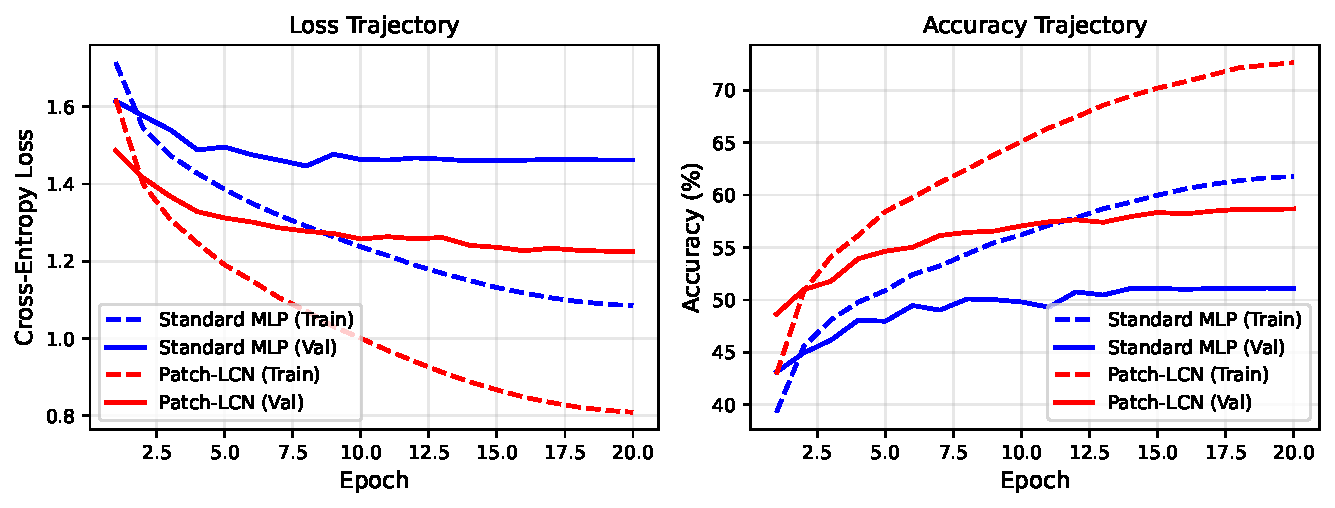
\includegraphics[width=0.78\linewidth]{figures/q1a_learning_curves.pdf}
\caption{Q1(a) Training and validation learning curves for Standard MLP vs. Patch-LCN over 20 epochs.}
\label{fig:q1a}
\end{figure}

\paragraph{Empirical Evidence and Scientific Nuance.}
As shown in Table~\ref{tab:q1a} and Figure~\ref{fig:q1a}, restricting first-layer receptive fields to $8 \times 8$ local spatial neighborhoods yields an immediate $+7.17\%$ test accuracy increase ($50.77\% \to 57.94\%$), even without translational weight sharing. 

However, from an epistemological perspective, we must state the precise scientific boundary of this comparison. Patch-LCN differs from the Standard MLP in two intertwined structural properties:
\begin{enumerate}
    \item \textbf{Local Connectivity Prior:} Pixel interactions are restricted to biologically plausible $8 \times 8$ neighborhoods.
    \item \textbf{Hierarchical Manifold Organization:} In Patch-LCN, the first layer produces $560$ activations ($16 \times 35$), preventing cross-patch linear combinations until the second layer. In the Standard MLP, cross-patch interactions occur immediately across all $3{,}072$ coordinates through a narrower 36-dimensional bottleneck.
\end{enumerate}
Thus, while this experiment conclusively refutes $H_2$ (proving that parameter starvation alone does not explain MLP failure), it isolates local spatial receptive fields jointly with block-structured covariance decoupling.

\subsection{Q1(b): Memorization Dynamics Under Label Noise}
\paragraph{Formulation and Effective Corruption Rate.}
To examine whether high-capacity networks learn genuine generalizable visual features before memorizing arbitrary labels, we deploy a High-Capacity MLP ($3{,}072 \to 512 \to 512 \to 10$, $1{,}841{,}162$ trainable parameters) providing $\sim 41$ parameters per training image.

We introduce label noise by selecting exactly $50\%$ of the training images ($22{,}500$ out of $45{,}000$) uniformly at random without replacement and re-assigning their labels via uniform sampling: $\tilde{y}_i \sim \text{Uniform}(\{0, \dots, 9\})$. 
Crucially, because uniform sampling over $K=10$ classes has a $1/K = 10\%$ probability of re-sampling the ground-truth label, the \textbf{effective label corruption rate} is:
\begin{equation}
    \eta_{\text{eff}} = \eta_{\text{nominal}} \times \left(1 - \frac{1}{K}\right) = 0.50 \times \left(1 - \frac{1}{10}\right) = 0.450 \quad (45.00\%).
\end{equation}
Specifically, exactly $20{,}250$ images ($45.00\%$) had their class labels altered, while $2{,}250$ selected images ($5.00\%$) chanced back to their true class, resulting in $55.00\%$ total clean labels in the training set. The $5{,}000$-sample validation set remained $100\%$ clean.

\begin{figure}[t]
\centering
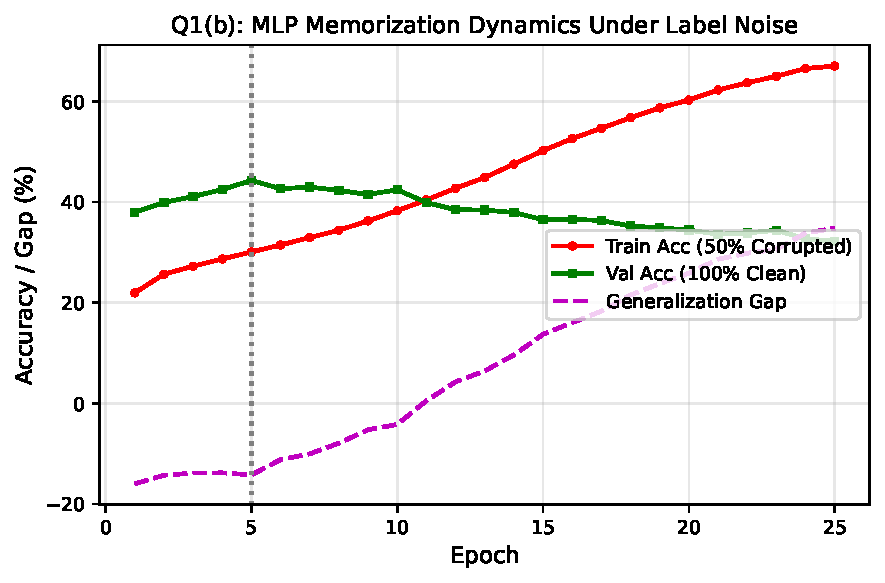
\includegraphics[width=0.78\linewidth]{figures/q1b_memorization_trajectory.pdf}
\caption{Q1(b) Memorization dynamics of High-Capacity MLP under 45\% effective label noise over 25 epochs. Clean validation accuracy peaks at Epoch 5 (44.30\%) before collapsing under active memorization.}
\label{fig:q1b}
\end{figure}

\begin{table}[t]
\centering
\caption{Q1(b) Trajectory checkpoints illustrating the transition from early visual learning to brute-force label fitting.}
\label{tab:q1b}
\resizebox{\columnwidth}{!}{
\begin{tabular}{ccccc}
\toprule
\textbf{Epoch} & \textbf{Train Acc (Noisy)} & \textbf{Val Acc (Clean)} & \textbf{Discrepancy} & \textbf{Phase Regime} \\
\midrule
$1$  & $28.53\%$ & $37.94\%$ & $-9.41\%$ & Coherent Feature Learning \\
$3$  & $35.80\%$ & $41.10\%$ & $-5.30\%$ & Spectral Alignment \\
$\mathbf{5}$  & $\mathbf{39.92\%}$ & $\mathbf{44.30\%}$ & $\mathbf{-4.38\%}$ & \textbf{Peak Generalization} \\
$8$  & $42.11\%$ & $42.30\%$ & $-0.19\%$ & Plateau Transition \\
$11$ & $42.47\%$ & $41.94\%$ & $+0.53\%$ & Trajectory Crossover \\
$15$ & $48.60\%$ & $38.10\%$ & $+10.50\%$ & Active Memorization \\
$20$ & $57.85\%$ & $34.50\%$ & $+23.35\%$ & Label Fitting \\
$25$ & $\mathbf{67.02\%}$ & $\mathbf{32.22\%}$ & $\mathbf{+34.80\%}$ & Overfitting Regime \\
\bottomrule
\end{tabular}
}
\end{table}

\begin{table}[t]
\centering
\caption{Q1(b) Comprehensive multi-subset accuracy audit on the saved checkpoint at Epoch 25 without retraining.}
\label{tab:q1b_audit}
\resizebox{\columnwidth}{!}{
\begin{tabular}{lcc}
\toprule
\textbf{Evaluated Partition / Subset} & \textbf{Sample Count ($N$)} & \textbf{Accuracy} \\
\midrule
1. Unselected Clean Train Subset & $22{,}500$ & $\mathbf{78.60\%}$ \\
2. Corrupted Train (vs. Noisy Assigned Target) & $22{,}500$ & $59.47\%$ \\
3. Corrupted Train (vs. True Ground Truth) & $22{,}500$ & $19.90\%$ \\
4. Clean Validation Set & $5{,}000$ & $32.22\%$ \\
\midrule
\textbf{True In-Distribution Gen Gap} (Row 1 $-$ Row 4) & — & $\mathbf{+46.38\%}$ \\
\textbf{Cross-Distribution Gap} (Row 2 $-$ Row 4) & — & $+27.25\%$ \\
\bottomrule
\end{tabular}
}
\end{table}

\paragraph{Analysis of Spectral Dynamics and Learning Trajectory.}
Tracking the optimization dynamics in Figure~\ref{fig:q1b} and Tables~\ref{tab:q1b} and~\ref{tab:q1b_audit} reveals three distinct phases:
\begin{enumerate}
    \item \textbf{Early Spectral Bias (Epochs 1--5):} Despite $45\%$ of training labels being corrupted, clean validation accuracy rises monotonically from $37.94\%$ to a peak of $\mathbf{44.30\%}$ at Epoch 5. Because true semantic visual patterns are shared across thousands of images, their stochastic gradients constructively align along low-frequency principal components, driving rapid early generalization.
    \item \textbf{Trajectory Crossover (Epoch 11):} At Epoch 11, training accuracy on noisy targets ($42.47\%$) surpasses clean validation accuracy ($41.94\%$), marking the boundary where gradient descent exhausts coherent signal and begins fitting unstructured noise.
    \item \textbf{Brute-Force Memorization (Epochs 12--25):} To fit random label noise, the network must memorize high-frequency sample-specific residuals~\cite{arpit2017closer}. By Epoch 25, training accuracy reaches $67.02\%$, while clean validation accuracy drops by $-12.08\%$ to $32.22\%$.
\end{enumerate}

\paragraph{Multi-Subset Audit and Generalization Gap Semantics.}
A crucial methodological distinction must be drawn regarding the generalization gap. When training on corrupted data, the difference $\text{TrainAcc}_{\text{noisy}} - \text{ValAcc}_{\text{clean}}$ is a \textit{cross-distribution transfer discrepancy} caused by synthetic distribution shift. 

Evaluating the checkpoint on individual subsets (Table~\ref{tab:q1b_audit}) establishes that the model achieves $\mathbf{78.60\%}$ accuracy on uncorrupted training examples and $\mathbf{59.47\%}$ on corrupted training targets, but collapses to $\mathbf{19.90\%}$ when predicting the true class of corrupted samples. The true in-distribution generalization gap on clean data is:
\begin{equation}
    \Delta_{\text{in-dist}} = \text{Acc}(S_{\text{clean\_train}}) - \text{Acc}(\mathcal{D}_{\text{val}}) = 78.60\% - 32.22\% = +46.38\%,
\end{equation}
demonstrating that memorizing $22{,}500$ random labels distorts the representation space, degrading clean feature generalization across all partitions.
